\chapter{Evaluación Primer Parcial}
\newpage

%\pagestyle{empty} 
\pagestyle{fancy} 


%-------------------------------------------------------------------------------
%-------------------------------------------------------------------------------
\topskip0pt
\vspace*{\fill}
{\centering
\section{Examen 1: Teórico/Oral/Investigaciones/Proyectos}}
\vspace*{\fill}

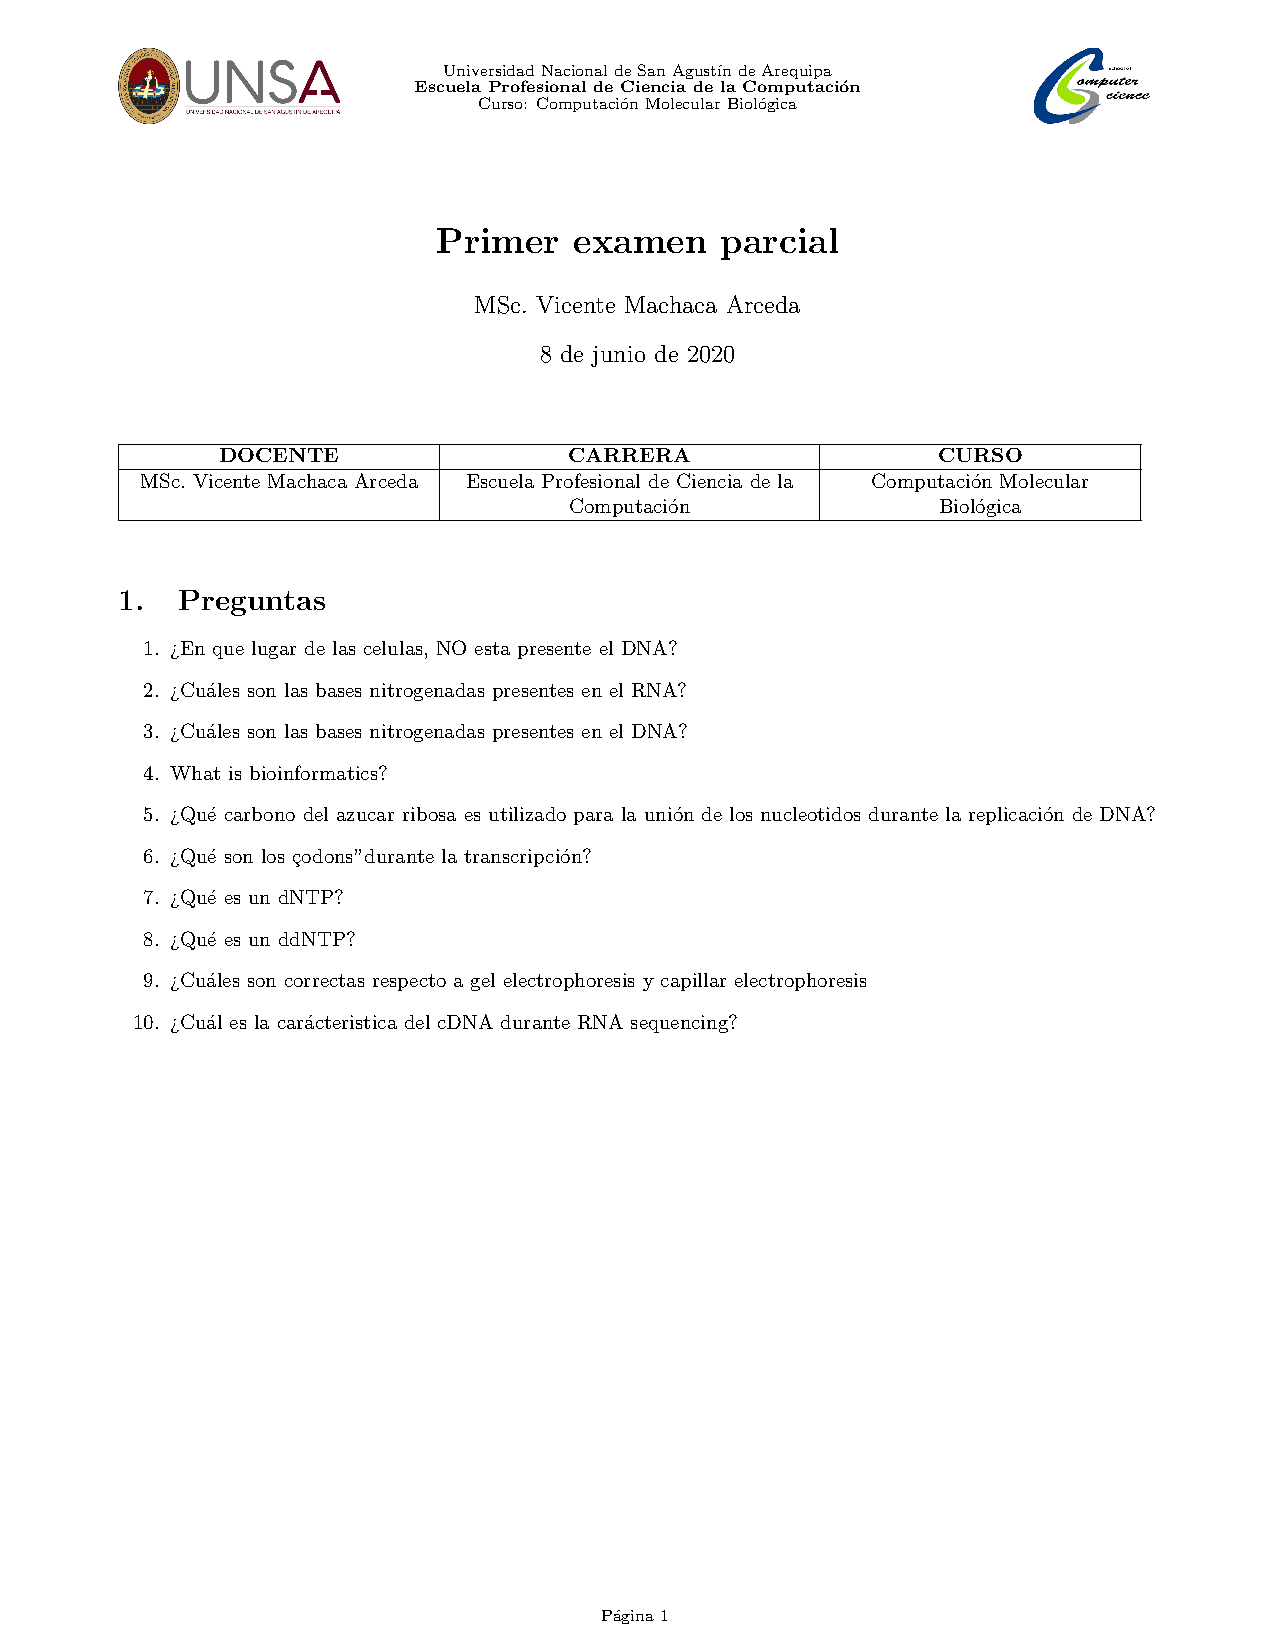
\includepdf[pages={1-}]{pdfs/7_examen_1.pdf}
%-------------------------------------------------------------------------------
%-------------------------------------------------------------------------------

%-------------------------------------------------------------------------------
%-------------------------------------------------------------------------------
\topskip0pt
\vspace*{\fill}
{\centering
\section{Resolución de la Examen 1}}
\vspace*{\fill}

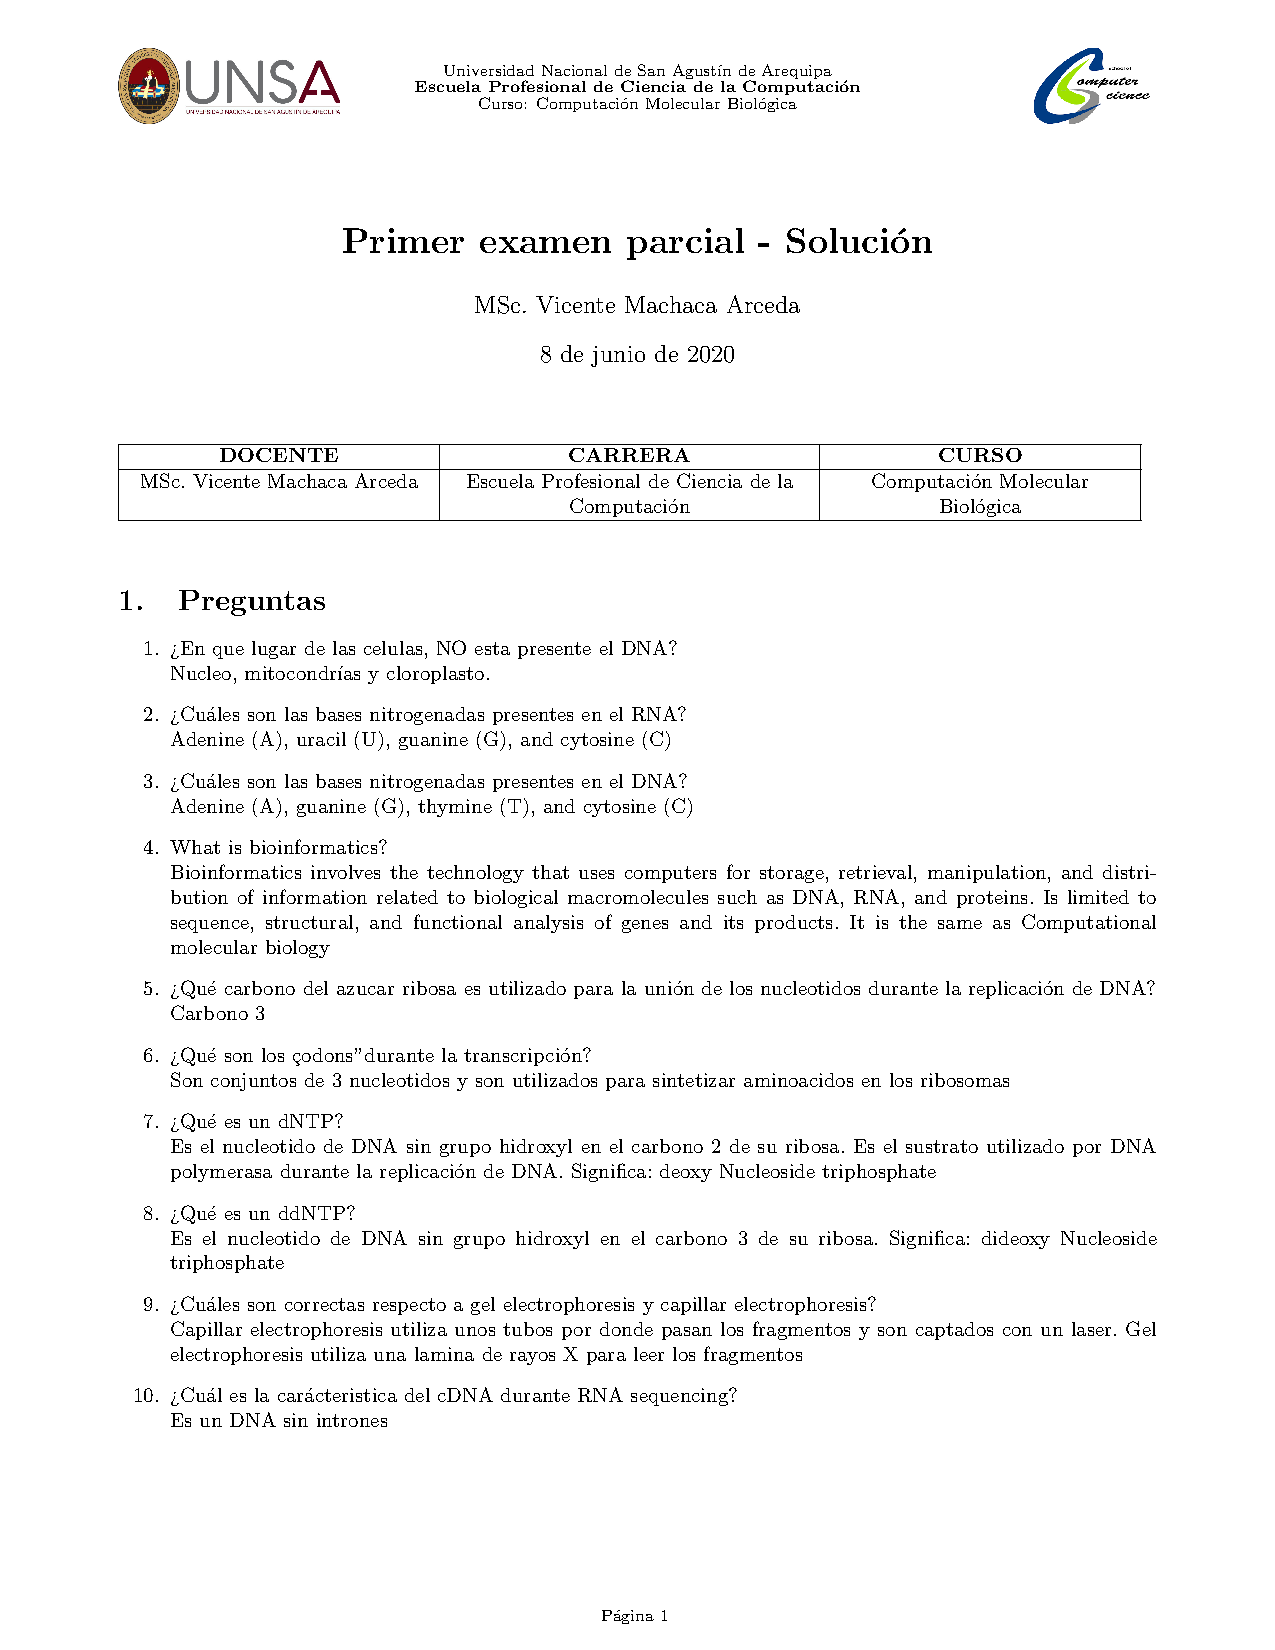
\includepdf[pages={1-}]{pdfs/7_examen_1_sol.pdf}
%-------------------------------------------------------------------------------
%-------------------------------------------------------------------------------


%-------------------------------------------------------------------------------
%-------------------------------------------------------------------------------
\clearpage
\topskip0pt
\vspace*{\fill}
{\centering
	\section{Evidencias}}
\vspace*{\fill}

\clearpage
\begin{table}[H]
	\centering
	\begin{tabular}{|x{\textwidth}|}
	\hline 
	\MakeUppercase{\csuniversidad} \\
	\\
	\begin{minipage}{.3\textwidth}
		
\includegraphics[width=\textwidth]{../imgs/cs2}
	\end{minipage} \\
	\\
	\textbf{\MakeUppercase{\csepcc}} \\
	\MakeUppercase{\csfacultad} \\
	\MakeUppercase{\csdepartamento} \\
	\hline 
	\end{tabular}
\end{table}

{\centering \textbf{EVIDENCIAS}}

\begin{flushleft}
	Los exámenes fueron tomados utilizando la plataforma Classroom, es así que estas evidencias están guardades en Google Drive. En la siguiente tabla presentamos dicho enlace.	
\end{flushleft}

\begin{table}[H]
	\centering
	\caption{Evidencias de los exámenes.}
	\begin{tabular}{|x{5cm}|x{2cm}|x{2cm}|x{3cm}|}
		\hline 
		\textbf{Descripción} & \textbf{Enlace} & \textbf{Nota} & \textbf{CUI} \\ \hline
		Exámenes & \href{https://docs.google.com/spreadsheets/d/1U4FTuQ_VT6xVcLQ_-JSvKlBPD5V_XOCM7DuyN5GfrUs/edit?usp=sharing}{Drive} & - & - \\  \hline		
		Nota promedio & \href{https://docs.google.com/spreadsheets/d/1U4FTuQ_VT6xVcLQ_-JSvKlBPD5V_XOCM7DuyN5GfrUs/edit?usp=sharing}{Drive} & 13 & - \\  \hline
		Mayor nota & \href{https://docs.google.com/spreadsheets/d/1U4FTuQ_VT6xVcLQ_-JSvKlBPD5V_XOCM7DuyN5GfrUs/edit?usp=sharing}{Drive} & 18 & 20160748 \\  \hline
		Menor nota & \href{https://docs.google.com/spreadsheets/d/1U4FTuQ_VT6xVcLQ_-JSvKlBPD5V_XOCM7DuyN5GfrUs/edit?usp=sharing}{Drive} & 2 & 20110202 \\  \hline
	\end{tabular}
\end{table}

%-------------------------------------------------------------------------------
%-------------------------------------------------------------------------------

%-------------------------------------------------------------------------------
%-------------------------------------------------------------------------------
\clearpage
\topskip0pt
\vspace*{\fill}
{\centering
\section{Informe Estadístico del mapeo del resultado del estudiante}}
\vspace*{\fill}
    
    \clearpage
    \begin{table}[H]
    \centering
		\begin{tabular}{|x{\textwidth}|}
			\hline 
            \MakeUppercase{\csuniversidad} \\
            \\
            \begin{minipage}{.3\textwidth}
				
\includegraphics[width=\textwidth]{../imgs/cs2}
	        \end{minipage} \\
        	\\
            \textbf{\MakeUppercase{\csepcc}} \\
            \MakeUppercase{\csfacultad} \\
            \MakeUppercase{\csdepartamento} \\
			\hline 
		\end{tabular}
	\end{table}


    %\begin{figure}				
	%			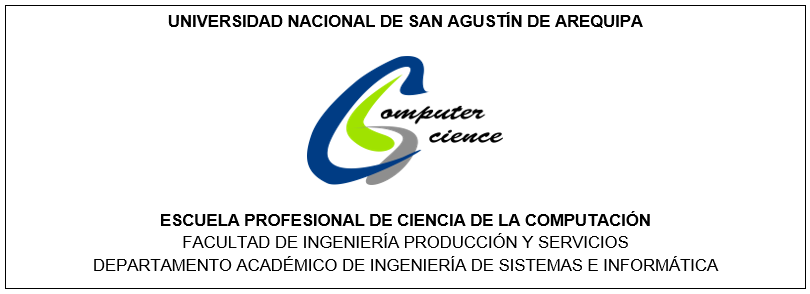
\includegraphics[width=\textwidth]{../imgs/cs}
	%\end{figure}
    \centering
    \textbf{INFORME DE RESULTADOS}    
        
    \begin{table}[H]
    \centering
		\begin{tabular}{|p{4cm}|p{2cm}|}
			\hline 
			\textbf{Nota máxima} & 18   \\
			\hline 
            \textbf{Nota mínima} & 2   \\
			\hline
			\textbf{Nota promedio} &  13   \\
			\hline 
		\end{tabular}
	\end{table}	
      
    \begin{flushleft}
    En la Figura \ref{fig:hist_EP1}, detallamos el histograma de frecuencias de las
    notas por grupo y en la Figura \ref{fig:hist_all_EP1}, mostramos el consolidado. 
    \end{flushleft}

    \begin{figure}[H]	
    \centering 		
				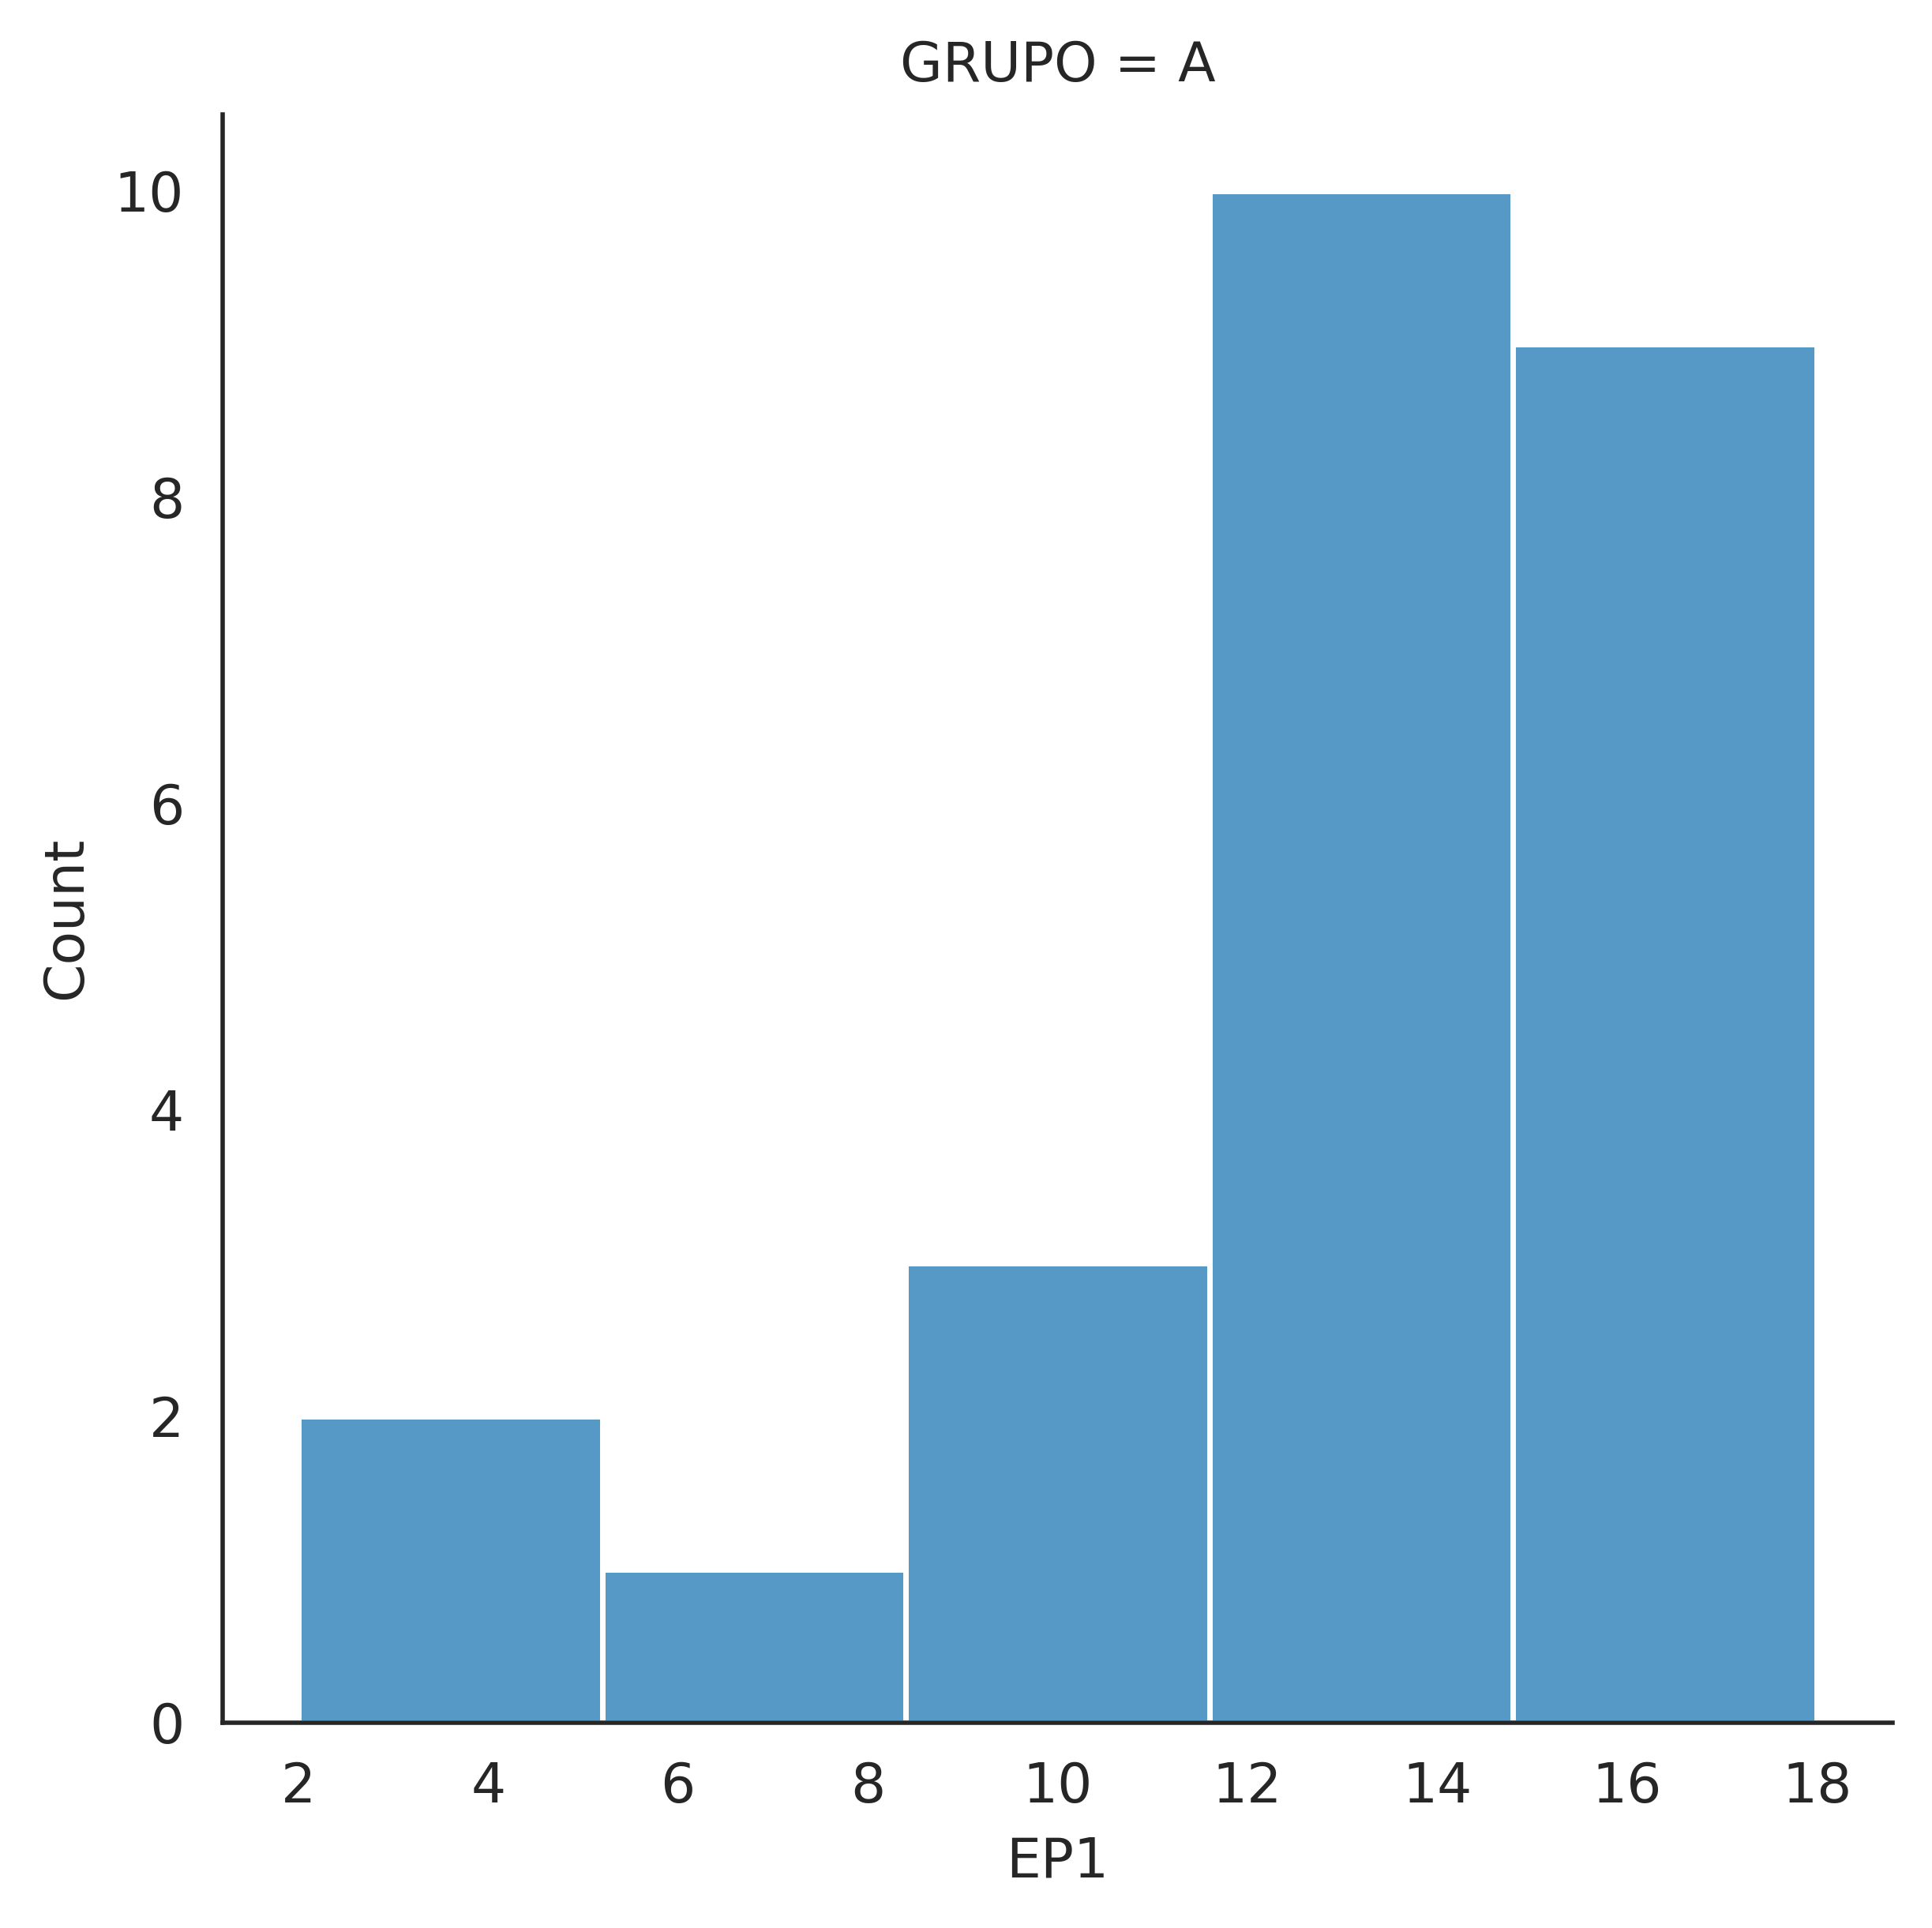
\includegraphics[width=0.6\textwidth]{../imgs/hist_EP1.png}
                \caption{Histograma de notas.}
                \label{fig:hist_EP1}
	\end{figure}

    \begin{figure}[H]	
    \centering 		
				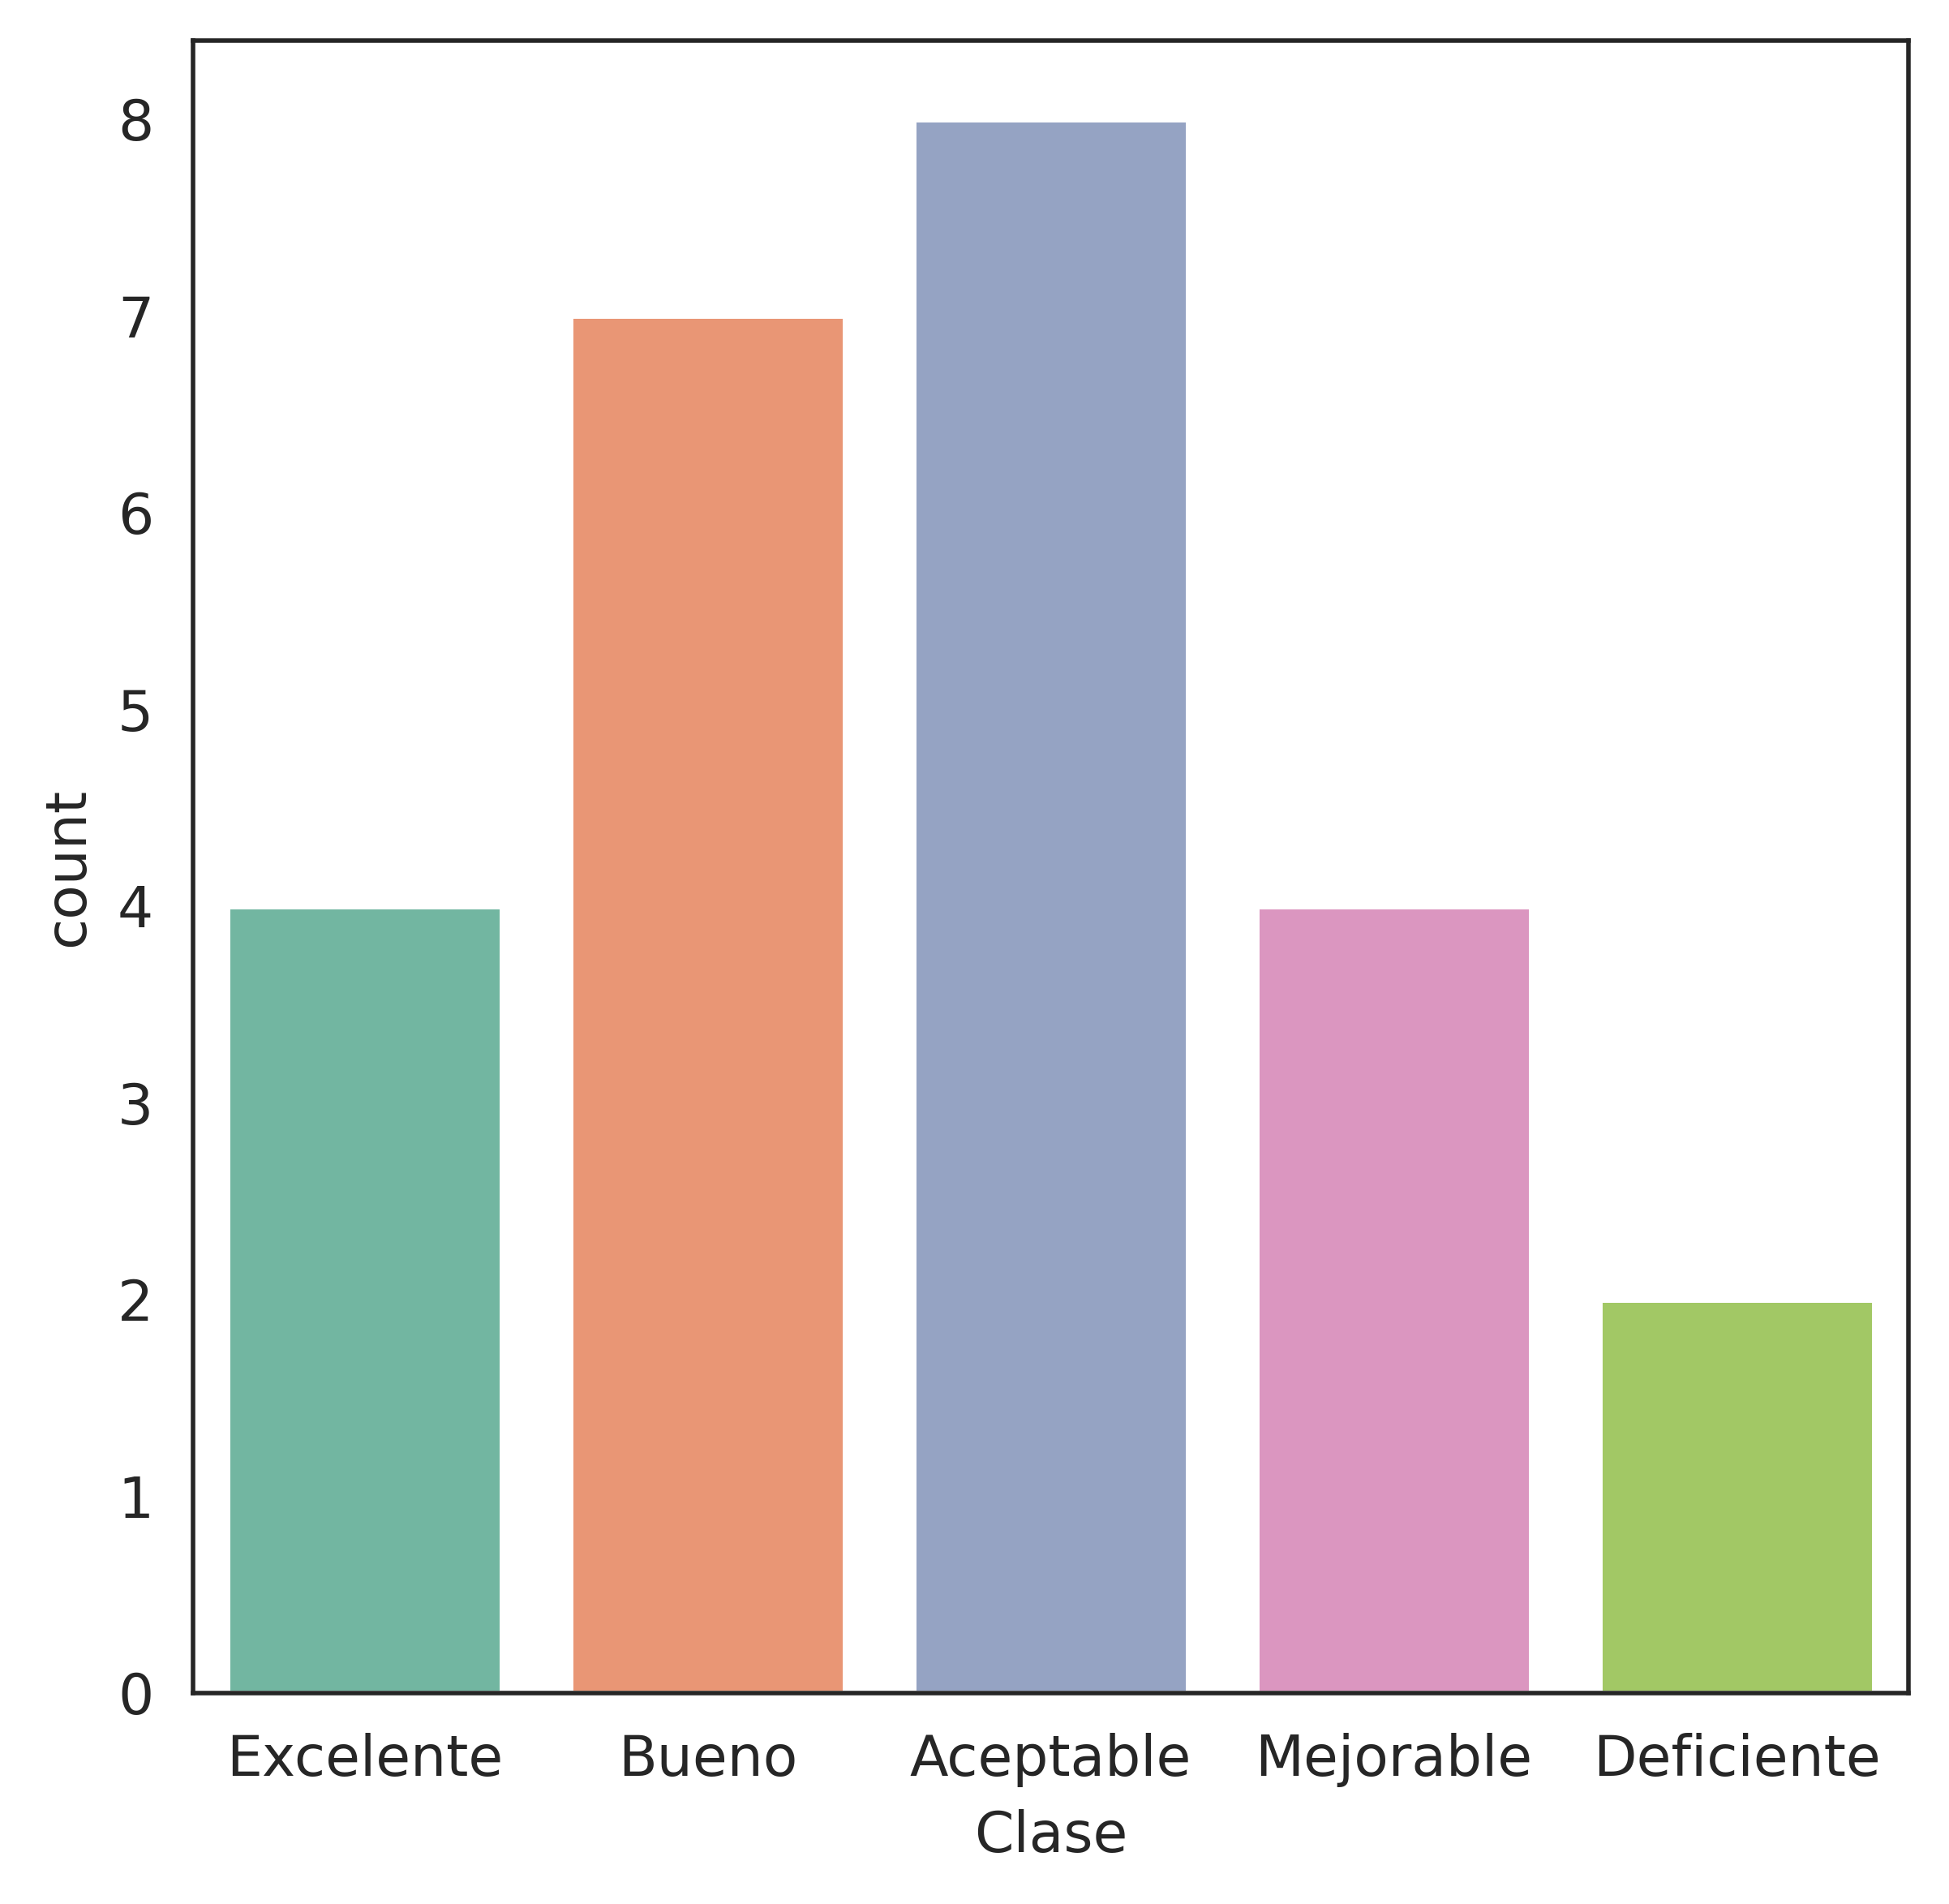
\includegraphics[width=0.6\textwidth]{../imgs/hist_all_EP1.png}
                \caption{Histograma de notas (consolidado). Excelente (nota $\geq$ 17), Bueno (14 $\leq$ nota $\leq$ 16), Aceptable (11 $\leq$ nota $\leq$ 13), Mejorable (07 $\leq$ nota $\leq$ 10), Deficiente ( nota $\leq$ 06)}
                \label{fig:hist_all_EP1}
	\end{figure}
      

        \begin{table}[H]
        \centering
            \caption{Notas del grupo A.}
            \begin{tabular}{|c|p{10cm}|c|}
                \hline 
                \textbf{CUI} & \textbf{ALUMNO} & \textbf{NOTA}  \\ \hline
        20153695 & APAZA CHAVEZ MARIA LOURDES & 15 \\ \hline 
            20143484 & AZA/MAMANI NICOLL DEL ROSARIO & 4 \\ \hline 
            20123493 & BARRIOS/CORNEJO SELENE & 14 \\ \hline 
            20123377 & BUSTINZA/CORNEJO ALEJANDRA PAMELA & 12 \\ \hline 
            20160748 & CESPEDES/FUENTES RENATO GONZALO & 18 \\ \hline 
            20143490 & CHUCTAYA/ELME MILAGROS & 9 \\ \hline 
            20132402 & CRUZ/MAMANI MILAGROS CELIA & 10 \\ \hline 
            20163436 & CUEVA/FLORES JONATHAN BRANDON & 12 \\ \hline 
            20052826 & ESPINEL QUISPE INGRID SALLY & 12 \\ \hline 
            20170734 & FERNANDEZ/MAMANI BRAYAN GINO & 14 \\ \hline 
            20173462 & GARCIA/DIAZ GERMAN FLAVIO & 16 \\ \hline 
            20163427 & GOMEZ/CONTRERAS JUNIOR VALENTIN & 8 \\ \hline 
            20143482 & GUTIERREZ/GUTIERREZ DIEGO ANTONY & 12 \\ \hline 
            20170732 & HERMOZA/LOAYZA MIGUEL ANGEL & 18 \\ \hline 
            20170735 & HERRERA/COOPER MIGUEL ALEXANDER & 13 \\ \hline 
            20160746 & INCA/CHIPANA GUSTAVO HERNAN & 10 \\ \hline 
            20151124 & NIFLA/CATASI WILLIAMS FIDEL & 13 \\ \hline 
            20160759 & OXA/CACYA SHIRLEY MICHELLE & 17 \\ \hline 
            20160750 & PANIBRA/MAMANI THALES GONZALO & 12 \\ \hline 
            20041749 & PILCO/PANCCA LUZ MARINA & 17 \\ \hline 
            20173453 & QUISPE/MENOR HERMOGENES & 16 \\ \hline 
            20153709 & QUISPE/QUISPE YARA JEANETTE & 12 \\ \hline 
            20110202 & TACORA/CRUZ RICHARD JAVIER & 2 \\ \hline 
            20173449 & TORRES/RODRIGUEZ JAIME FRANCISCO & 16 \\ \hline 
            20170737 & VICENTE/CASTRO RENZO OMAR & 16 \\ \hline 
            		
            \end{tabular}
        \end{table}	
        
%-------------------------------------------------------------------------------
%-------------------------------------------------------------------------------

%-------------------------------------------------------------------------------
%-------------------------------------------------------------------------------
\clearpage
\topskip0pt
\vspace*{\fill}
{\centering
	\section{Lista de Cotejos del proceso de Evaluación Parcial}}
\vspace*{\fill}

\clearpage
\begin{table}[H]
	\centering
	\begin{tabular}{|x{\textwidth}|}
	\hline 
	\MakeUppercase{\csuniversidad} \\
	\\
	\begin{minipage}{.3\textwidth}
		
\includegraphics[width=\textwidth]{../imgs/cs2}
	\end{minipage} \\
	\\
	\textbf{\MakeUppercase{\csepcc}} \\
	\MakeUppercase{\csfacultad} \\
	\MakeUppercase{\csdepartamento} \\
	\hline 
	\end{tabular}
\end{table}

\vspace{1cm}
{\centering 
\MakeUppercase{\textbf{Asignatura}}: \MakeUppercase{\cscourse}} \\
\vspace{0.5cm}

\begin{table}[H]
	\centering
	\begin{tabular}{|x{\textwidth}|}
		\hline 
		\cellcolor{light_gray} \textbf{LISTA DE COTEJO Y PROCESO DE EVALUACIÓN} \\ \hline
	\end{tabular}
\end{table}

\begin{table}[H]
	\centering
	\begin{tabular}{|p{0.4\textwidth}|p{0.575\textwidth}|}
		\hline 
		\textbf{Docente} & \csauthor \\ \arrayrulecolor{black}\hline
		\textbf{Categoría/Regimen} & \cscategoria / \csregimen \\ \hline
		\textbf{Semestre} & \cssemestre \\ \hline
		\textbf{Fecha} & 26 de Mayo \\ \hline
	\end{tabular}
\end{table}

\begin{table}[H]
	\centering
	\begin{tabular}{|p{0.4cm}|p{4.8cm}|p{1.3cm}|p{5cm}|p{1.8cm}|}
		\hline 
		\textbf{N$^{\circ}$} & \textbf{Examen} & \textbf{Puntaje} & \textbf{Comentario} & \textbf{Porcentaje} \\ \hline
		1 & Examen de conocimientos & 20 & Opción multiple y respuestas cortas & 15\% \\ \hline
		\multicolumn{4}{|r|}{\textbf{TOTAL}} & 20 \\ \hline
		\multicolumn{4}{|r|}{\textbf{TOTAL PORCENTAJE}} & 15\% \\ \hline
	\end{tabular}
\end{table}
%-------------------------------------------------------------------------------
%-------------------------------------------------------------------------------

%-------------------------------------------------------------------------------
%-------------------------------------------------------------------------------
\clearpage
\topskip0pt
\vspace*{\fill}
{\centering
	\section{Porcentaje de avance y último contenido desarrollado de acuerdo a silabo}}
\vspace*{\fill}

\clearpage
\begin{table}[H]
	\centering
	\begin{tabular}{|x{\textwidth}|}
	\hline 
	\MakeUppercase{\csuniversidad} \\
	\\
	\begin{minipage}{.3\textwidth}
		
\includegraphics[width=\textwidth]{../imgs/cs2}
	\end{minipage} \\
	\\
	\textbf{\MakeUppercase{\csepcc}} \\
	\MakeUppercase{\csfacultad} \\
	\MakeUppercase{\csdepartamento} \\
	\hline 
	\end{tabular}
\end{table}

\vspace{1cm}
{\centering 
	\MakeUppercase{\textbf{Asignatura}}: \MakeUppercase{\cscourse}} \\
\vspace{0.5cm}

\begin{table}[H]
	\centering
	\begin{tabular}{|x{\textwidth}|}
		\hline 
		\cellcolor{light_gray} \textbf{PORCENTAJE DE AVANCE Y ÚLTIMO CONTENIDO DESARROLLADO} \\ \hline
	\end{tabular}
\end{table}

\begin{table}[H]
	\centering
	\begin{tabular}{|p{0.4\textwidth}|p{0.575\textwidth}|}
		\hline 
		\textbf{Docente} & \csauthor \\ \arrayrulecolor{black}\hline
		\textbf{Categoría/Regimen} & \cscategoria / \csregimen \\ \hline
		\textbf{Semestre} & \cssemestre \\ \hline
		\textbf{Fecha} & 26 de Mayo \\ \hline
	\end{tabular}
\end{table}

\begin{table}[H]
	\centering
	\begin{tabular}{|p{0.4cm}|p{2.5cm}|p{2.6cm}|p{8.3cm}|}
		\hline 
		\textbf{N$^{\circ}$} & \textbf{Fecha} & \textbf{Porcentaje} & \textbf{Contenido} \\ \hline
		1 & 13 de Mayo & 30\% & Alineamiento de secuencias \\ \hline
	\end{tabular}
\end{table}
%-------------------------------------------------------------------------------
%-------------------------------------------------------------------------------

